\documentclass{lug}
\usepackage{graphicx}
\usepackage{amsmath}
\usepackage{bm}
\usepackage{xcolor}
\usepackage{pseudocode}
\usepackage{romannum}

\title{A Parallel Implementation of Random Forest}
\author{Lou Brand and Xun Li}
\institute{\textbf{Department of Computer Science\\Colorado School of Mines}}
\date{\today}

\begin{document}

\section{Background}
\frame{
    \frametitle{Random Forest}
    \begin{center}
        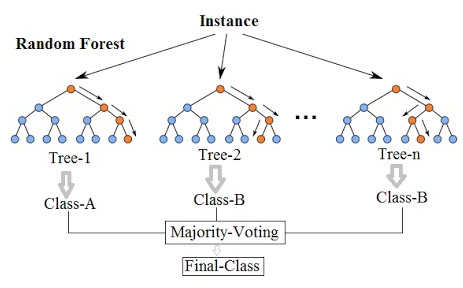
\includegraphics[scale=0.6]{images/random-forest-simplified.jpg}\\
    \end{center}
}

\frame{
    \frametitle{gcForest}
    \begin{center}
        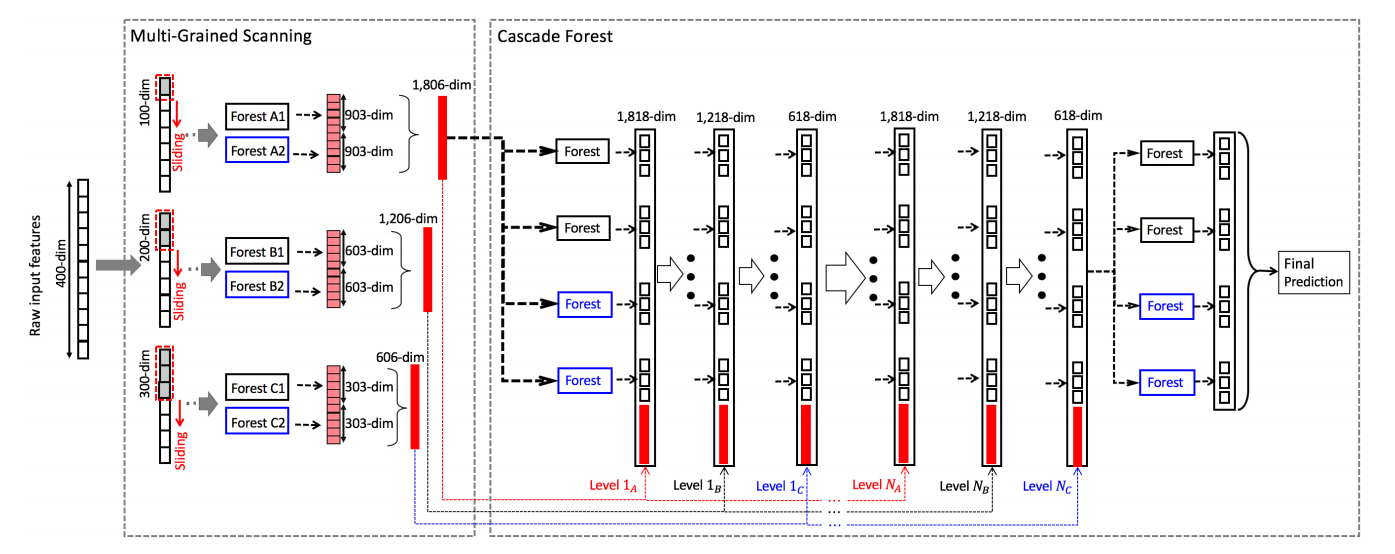
\includegraphics[scale=0.3]{images/gcForest.png}\\
        ``The efficiency of gcForest can be improved further with optimized parallel implementation'' - \textit{Zhou et. al.}
    \end{center}
}
\frame{
    \frametitle{Applications}
    \begin{center}
        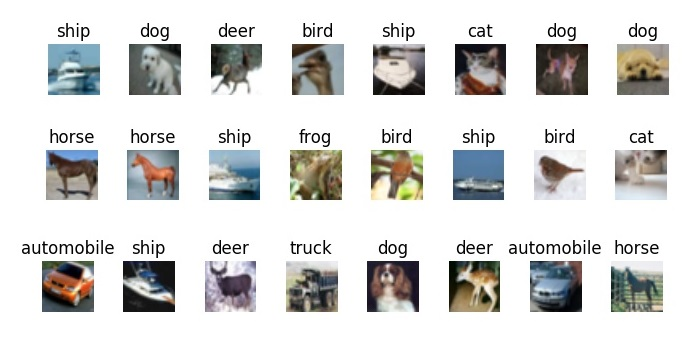
\includegraphics[scale=0.75]{images/cifar1.jpg}\\ 
        Face perception, image tagging, regression, classification, etc.
    \end{center}
}

\frame{
    \frametitle{An Insight into Node Splitting}
    \begin{itemize}[<+->]
        \item The elemental operation of the random forest algorithm
        \item More interesting than the embarassingly parallelism mentioned in gcForest
        \item Tree algorithms are inherently difficult to parallelize
            \begin{enumerate}
                \item Load balancing
                \item Dynamic irregular memory accesses
                \item As we further down in the tree we use many small kernels
            \end{enumerate}
    \end{itemize}
}

\section{Approach}
\frame{
    \frametitle{Node Splitting}
    \begin{center}
        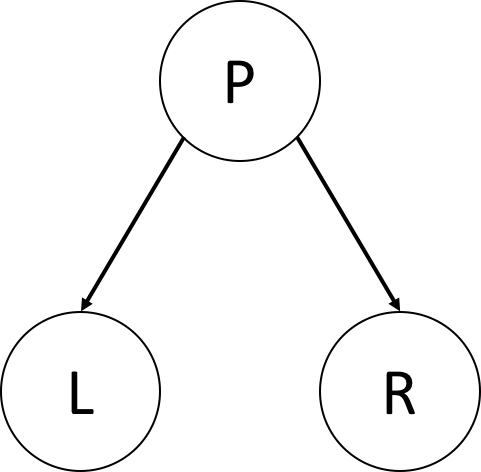
\includegraphics[scale=0.5]{images/node-split.png}\\
        \textbf{Goal}: Optimize splitting of the nodes using parallel programming techniques 
    \end{center}
}

\frame{
    \frametitle{Maximize Information Gain}
    \begin{enumerate}[<+->]
        \item Choose a $feature$ to split on 
        \item Organize data samples into L and R children nodes 
        \item Calculate information gain: 
            $$ IG_{feature}=GI_P-\frac{N_L}{N}GI_L-\frac{N_R}{N}GI_R $$
        where,
            $$ GI=1- \sum_{j=0}^{M}(\frac{C_j}{W})^2 $$
        $W$ samples in parent node, $C_j$ number of samples w/ label $j$
        \item Repeat 1-3 for additional features
        \item Splitting feature $= argmax(IG_{feature})$
    \end{enumerate}
}

\section{Implementation and Experiments}

\frame{
    \frametitle{Experimental Setup}
    \textbf{Synthetic Data}
    \begin{enumerate}
        \item Dataset size: 8,388,608 samples 
        \item Feature range: 3,200 discrete values
        \item Labels: 32 classes
    \end{enumerate}
    \pause
    \textbf{Environment} Intel Xeon ES-2670
    \begin{enumerate}
        \item 8x hyper-threads (4 cores)
    \end{enumerate}
    \pause
    \textbf{Environment} NVIDIA GRID GPU (Kepler GK104)
    \begin{enumerate}
        \item Memory: 2 GB
        \item Memory bandwidth: 224.3 GB/sec
    \end{enumerate}
}

\frame{
    \frametitle{CPU Baseline}
    \begin{center}
        \Large{\textbf{Serial:} 94970 ms\\ \textbf{OpenMP:} 16773 ms}
    \end{center}
}

\frame{
    \frametitle{GPU Implementation--Atomic Block}
    \begin{center}
        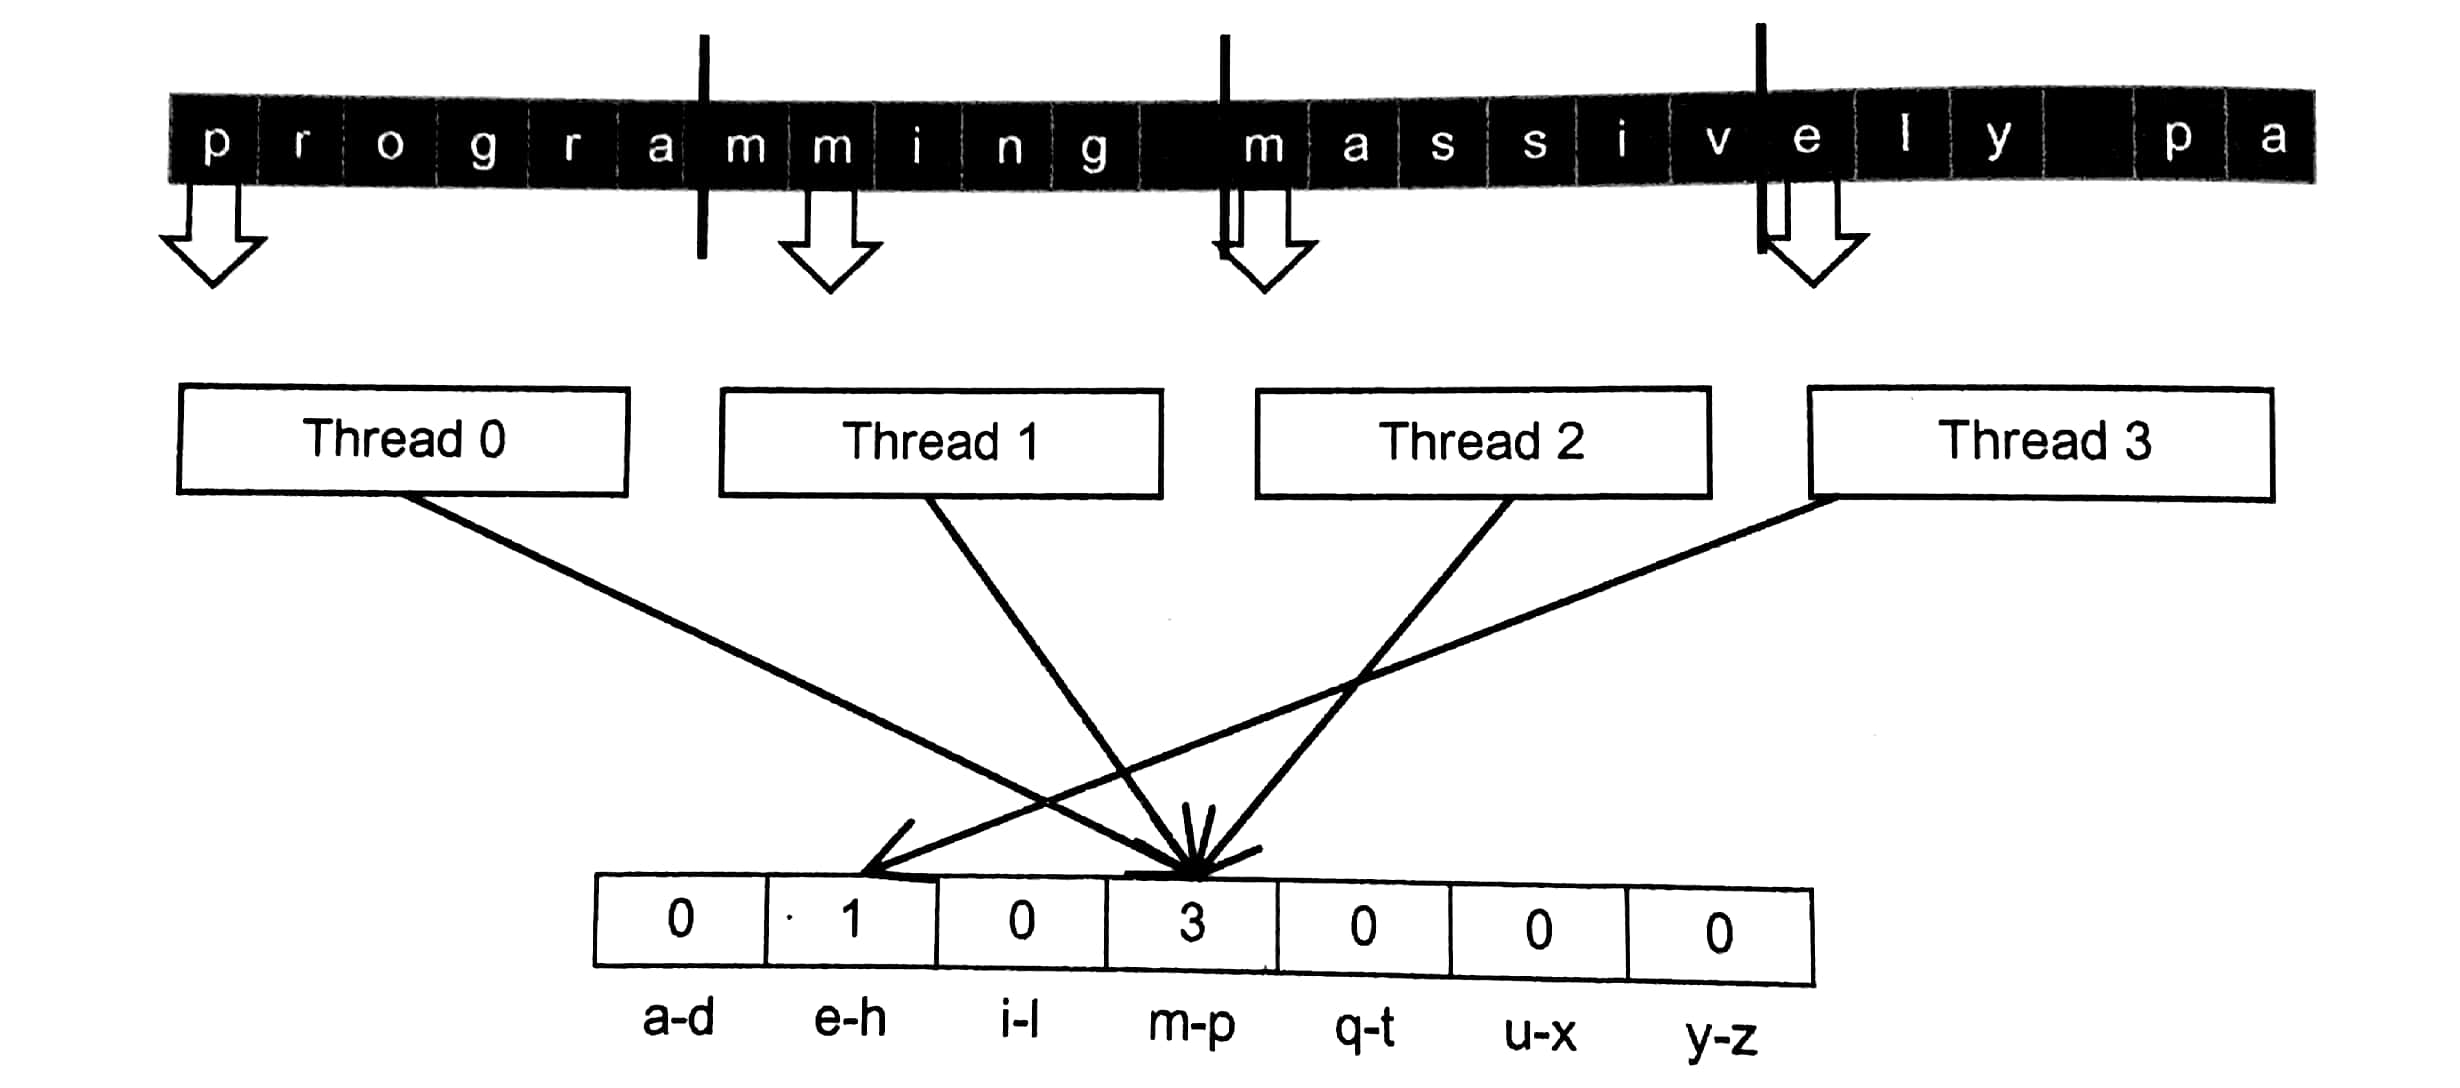
\includegraphics[scale=.12]{images/parallel-histogram.jpg}
    \end{center}
}

\frame{
    \frametitle{GPU Implementation--Atomic Block} 
    \begin{center}
        \Large{\textbf{Atomic Block:} 43422 ms\\ \textbf{Atomic Throughput:} 4.06 GB/sec (on GT 750M) out of 80 GB/sec}
    \end{center}
}

\frame{
    \frametitle{GPU Implementation--Atomic Interleaved}
    \begin{center}
        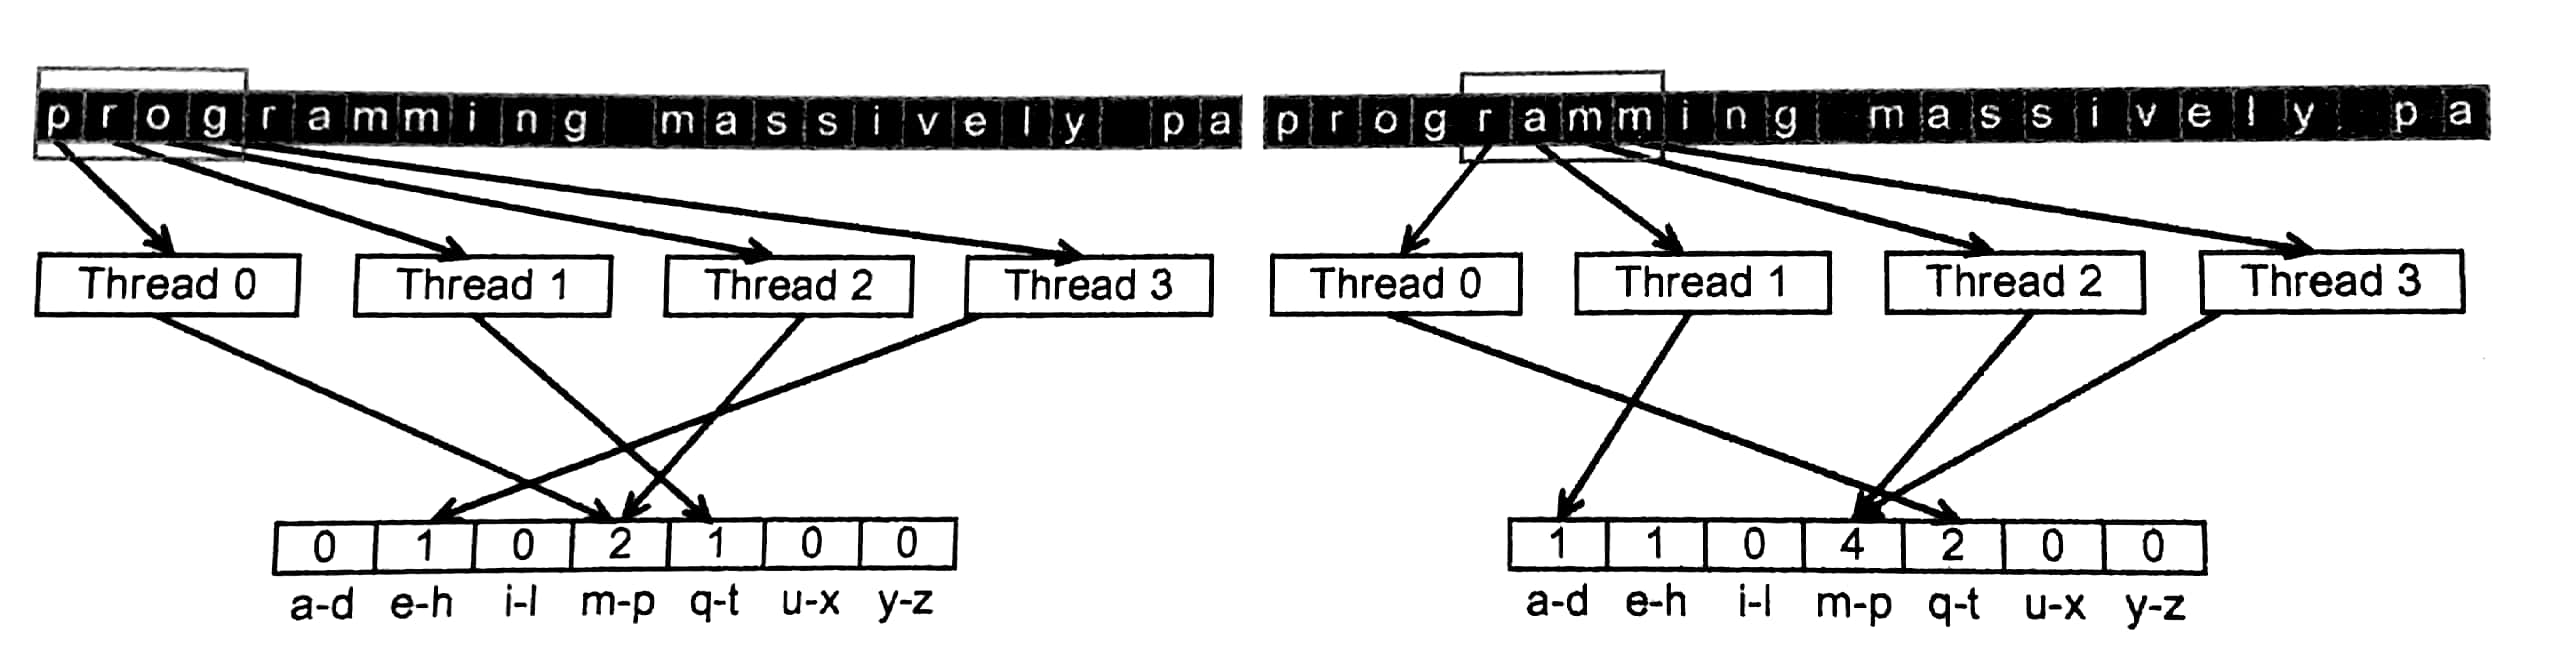
\includegraphics[scale=.13]{images/interleaved.jpg}
    \end{center}
}

\frame{
    \frametitle{GPU Implementation--Atomic Interleaved}
    \begin{center}
        \Large{\textbf{Atomic Interleaved:} 8573 ms\\ \textbf{Atomic Throughput:} 18.6 GB/sec (on GT 750M) out of 80 GB/sec}
    \end{center}
}

\frame{
    \frametitle{GPU Implementation--Atomic Privatization}
    \begin{center}
        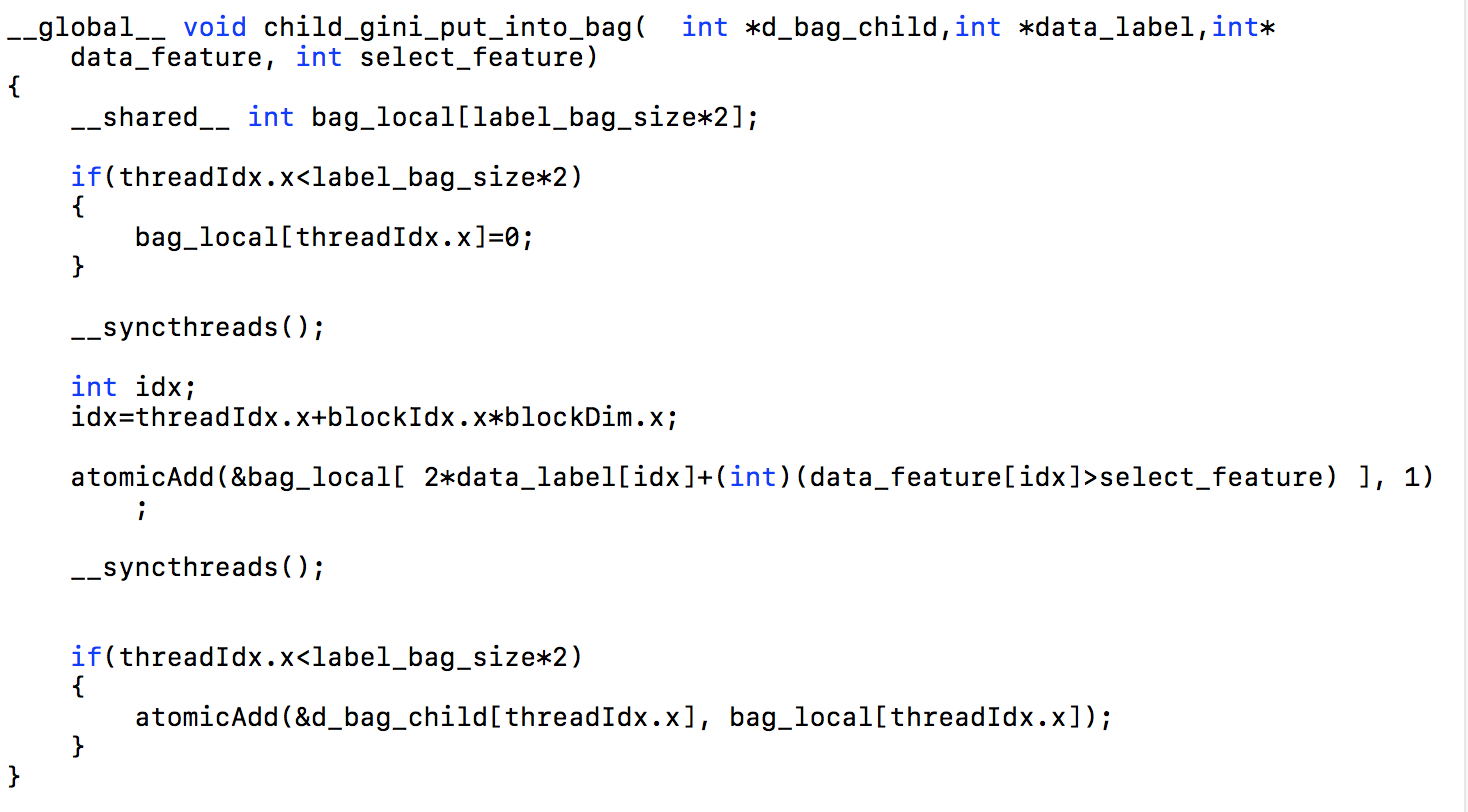
\includegraphics[scale=.45]{images/privitization-code.png}
    \end{center}
} 

\frame{
    \frametitle{GPU Implementation--Atomic Privatization}
    \begin{center}
        \Large{\textbf{Atomic Privatization:} 5288 ms\\ \textbf{Atomic Throughput:} 1.07 GB/sec (on GT 750M) out of 80 GB/sec}
    \end{center}
}

\frame{
    \frametitle{GPU Implementation--Coarse-Grained Parallelism}
    \begin{pseudocode}{SplittingNode}{label,feature,S} 
        1\color{red}{\quad \FOR k \GETS 0 \TO max(S)}\\
    2\quad	 \quad \FOR i \GETS 0 \TO N \\
        3\quad \quad \text{Compute Histogram}\\
        4\quad \quad  N, N_L, N_R \GETS sum(b_P),sum(b_L),sum(b_R)\\
        5\quad \quad \text{Compute:} \quad GI_P, GI_L, GI_R\\
        6\quad \quad \text{Compute:} \quad IG[k]\\
    7\quad \quad split \GETS S[argmax(IG)]\\
    8\quad \RETURN{split, child}
    \end{pseudocode}
}


\frame{
    \frametitle{GPU Implementation--Coarse-Grain Parallelism} 
    \begin{center}
        \Large{\textbf{Coarse-Grain:} 5226 ms}
    \end{center}

}

\section{Insights}

\frame{
    \frametitle{What Should We Choose?}
    \textbf{Some Intuition}
    \begin{itemize}[<+->]
        \item GPU computation works well early on in the tree (when there are many instances to be bagged)
        \item Further down the tree the CPU implementation works best
    \end{itemize}
    \textbf{What to Choose}
    \begin{itemize}[<+->]
    	\item CPU Serial: ``Smaller'' Datasets
        \item CPU Parallel (OpenMP): ``Small'' Datasets
        \item GPU Privatization: ``High Contention'' Datasets
        \item GPU Coarse-Grain: ``Large Number of Features'' Datasets
    \end{itemize}
}

\frame{
    \frametitle{Future Work}
    \textbf{Algorithmic Changes to Improve Redundancy}
    \begin{enumerate}[<+->]
        \item The first node split can be precomputed and stored
        \item Pooling some tasks via node merge, helps with load balance issues 
        \item Pipe-lining with CPU and GPU
    \end{enumerate}
}

\frame{
    \frametitle{Conclusions}
    \textbf{What Did We Learn?}
    \begin{itemize}[<+->]
        \item Six implementations of node splitting (CPU/GPU)
        \item Deeper understanding of the performance bottlenecks
        \item Insights into the random forest optimization at a fine and coarse-grained level 
    \end{itemize}
}

\frame{
    \begin{center}
        \Huge{Questions/Discussion}\\
    \end{center}
}

\nocite{*} % Include everything in the .bib file.
\bibliographystyle{plainnat}
\bibliography{random-forest-gpu}

% that's all, folks
\end{document}
